\documentclass[11pt,letterpaper]{article}
\usepackage[lmargin=1in,rmargin=1in,tmargin=1in,bmargin=1in]{geometry}
\usepackage{../../style/homework}
\setbool{quotetype}{true} % True: Side; False: Under
\setbool{hideans}{false} % Student: True; Instructor: False

% -------------------
% Content
% -------------------
\begin{document}

\homework{2: Due 02/01}{You say impossible, but all I hear is, `I'm possible.'\,}{Ted Lasso, Ted Lasso}

% Problem 1
\problem{10} Showing all your work and fully justifying your reasoning, compute the following:
	\begin{2enumerate}
	\item $\ds \lim_{x \to 0} \dfrac{\sin(3x)}{\cos(5x)}$
	\item $\dfrac{d}{dx}\, \left( \dfrac{x e^x}{x^2 + 1} \right)$
	\item $\dfrac{d^2}{dx^2} (x^2 + 5)^{10}$
	\item $\ds \int x e^x \; dx$
	\end{2enumerate} \pspace

\sol 
\begin{enumerate}[(a)]
\item 
	\[
	\lim_{x \to 0} \dfrac{\sin(3x)}{\cos(5x)}= \dfrac{\sin(0)}{\cos(0)}= \dfrac{0}{1}= 0
	\]

\item 
	\[
	\dfrac{d}{dx}\, \left( \dfrac{x e^x}{x^2 + 1} \right)= \dfrac{(x^2 + 1)(e^x + xe^x) - (2x)(xe^x)}{(x^2 + 1)^2}= \dfrac{e^x \big((x^2 + 1)(1 + x) - 2x^2 \big)}{(x^2 + 1)^2}= \dfrac{e^x (x^3 - x^2 + x + 1)}{(x^2 + 1)^2}
	\]

\item 
	\[
	\begin{aligned}
	\dfrac{d}{dx}\, (x^2 + 5)^{10}&= 10(x^2 + 5)^9 \cdot 2x= 20x (x^2 + 5)^9 && \\[0.3cm]
	\dfrac{d^2}{dx^2} (x^2 + 5)^{10}&= \dfrac{d}{dx} \left( \dfrac{d}{dx} (x^2 + 5)^{10} \right)= \dfrac{d}{dx} \left( 20x (x^2 + 5)^9 \right) \hspace{-0.3cm} &&= 20(x^2 + 5)^9 + 20x \cdot \big( 9(x^2 + 5)^8 \cdot 2x \big) \\
	&&&= 20(x^2 + 5)^9 + 360x^2 (x^2 + 5)^8 \\
	&&&= 20(x^2 + 5)^8 (19x^2 + 5)
	\end{aligned}
	\]

\item 
	\[
	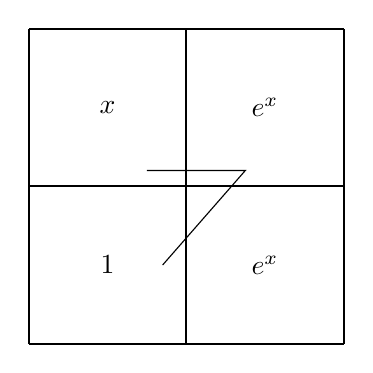
\begin{tikzpicture}
	\draw[thick] (0,0) -- (4,0);
	\draw[thick] (4,0) -- (4,4);
	\draw[thick] (4,4) -- (0,4);
	\draw[thick] (0,4) -- (0,0);
	\draw[thick] (2,0) -- (2,4);
	\draw[thick] (0,2) -- (4,2);
	\node at (1,3) {$x$};
	\node at (1,1) {$1$};
	\node at (3,1) {$e^x$};
	\node at (3,3) {$e^x$};
	\draw (1.5,2.2) -- (2.75,2.2) -- (1.7,1);
	\end{tikzpicture}
	\]
	\[
	\int xe^x \;dx= xe^x - \int e^x \;dx= xe^x - e^x + C
	\]
\end{enumerate}



\newpage 



% Problem 2
\problem{10} One of the first `non-trivial' approximation techniques one learns is the process of linearization. Recall that if $f(x)$ is differentiable at $c$, the linearization of $f(x)$ at $c$, denoted $L(x)$, is the tangent line of $f(x)$ at $x= c$. But then for $x \approx c$, we have $f(x) \approx L(x)$. Consider the function $f(x)= \sqrt{x}$. 
	\begin{enumerate}[(a)]
	\item Find the linearization of $f(x)$ at $x= 144$. 
	\item Use (a) to approximation $\sqrt{150}$. What is the error for your approximation?
	\item Is this generally a useful method for computing $f(x)= \sqrt{x}$? Explain. 
	\end{enumerate} \pspace

\sol 
\begin{enumerate}[(a)]
\item The linearization of $f(x)$ at $x= 144$ is the tangent line of $f(x)$ at $x= 144$. We have\dots
	\[
	\begin{aligned}
	f(144)&= \sqrt{144}= 12 \\[0.3cm]
	f'(x)&= \dfrac{1}{2\sqrt{x}} \Rightarrow f'(144)= \dfrac{1}{2 \sqrt{144}}= \dfrac{1}{24}
	\end{aligned}
	\]
The linearization is then\dots
	\[
	L(x)= f(144) + f'(144) \big(x - 144\big)= 12 + \dfrac{1}{24} \big(x - 144\big)= \dfrac{x}{24} + 6
	\] 

\item We have\dots
	\[
	\sqrt{150}= f(150) \approx L(150)= 12 + \dfrac{1}{24} \big(150 - 144 \big)= 12 + \dfrac{6}{24}= 12 + \dfrac{1}{4}= 12.25
	\]
We know that $\sqrt{150} \approx 12.2474$. The error in the approximation is then $|12.2474 - 12.25|= 0.0026$ and the relative error is $\frac{|12.2474 - 12.25|}{|12.2474|}= 2.12\%$. 

\item The approximation in (b) requires us to be able to construct the tangent line to $f(x)= \sqrt{x}$ at $x= c$, which required us to know $f(c)$. But then we require $c$ to be a perfect square. Then to approximate $\sqrt{r}$, we need $r$ to be `close' to a perfect square. However, as $n \to \infty$, the difference between the $n$th perfect square and the $(n+1)$th perfect square tends to infinity. Therefore for `most' $r$, $r$ will not be `close' to a perfect square. It is then likely that for such $r$, $\sqrt{r} = f(r) \not\approx L(r)$.\footnote{This is offset by the fact that $f'(x)= \frac{1}{2\sqrt{x}} \to 0$ as $x \to \infty$, so that the fact that $r$ and nearest perfect square might have a large difference might be offset. In fact, this is still not the case. Suppose that $c= n^2$ is a perfect square. The difference between $c$ and the next perfect square is $(n + 1)^2 - n^2= 2n + 1$. Suppose $r$ is one of the integers closest to $\frac{(n + 1)^2 + n^2}{2}= \frac{2n^2 + 2n + 1}{2}= n^2 + n + \frac{1}{2}$, i.e. $n^2 + n$ or $n^2 + n + 1$. The tangent line to $f(x)$ at $x= n^2$ is $L(x)= f(n^2) + f'(n^2) (x - n^2)= n + \frac{1}{2n} (x - n^2)$. Take $r= n^2 + n$. Then $L(r)= L(n^2 + n)= n + \frac{1}{2n} (n^2 + n - n^2)= n + \frac{1}{2}$. So if $r$ is large (so that $n$ must too be large), this has error $|\sqrt{r} - L(r)|= |\sqrt{n^2 + n} - n - \frac{1}{2}|= |\sqrt{n^2(1 + \frac{1}{n})} - n - \frac{1}{2}|= |n \sqrt{1 + \frac{1}{n}} - n - \frac{1}{2}| \approx |n \sqrt{1 + 0} - n + \frac{1}{2}|= |n - n + \frac{1}{2}|= \frac{1}{2}$. But then we cannot use the linearization to approximate $\sqrt{r}$ for values between `large' perfect squares with arbitrary accuracy.}
\end{enumerate}



\newpage



% Problem 3
\problem{10} Another of the first `non-trivial' approximation techniques one learns is Taylor series. The Taylor series of a function can be used to approximate values of the function. In fact, the (infinite) Taylor series can be exactly equal to the function. Consider the polynomial $f(x)= x^3 - 5x^2 + 7$. 
	\begin{enumerate}[(a)]
	\item Find the Taylor Series for $f(x)$ at $x= 1$. 
	\item Show your Taylor Series in (a) is exactly $f(x)$. 
	\item Assuming that $(x - 1)^n$ is `negligible' whenever $n > 1$ and $x \approx 1$, use (b) to approximate $f(1.01)$. What is the error for this approximation? 
	\end{enumerate} \pspace

\sol 
\begin{enumerate}[(a)]
\item Recall that the Taylor series of $f(x)$ at $x= c$ (if it exists) is $\ds \sum_{n=0}^\infty \dfrac{f^{(n)}(c)}{n!} \, (x - c)^n$. We have\dots
	\[
	\begin{aligned}
	f(1)&= 1 - 5 + 7= 3 \\
	f'(x)&= 3x^2 - 10x \Rightarrow f'(1)= 3 - 10= -7 \\
	f''(x)&= 6x - 10 \Rightarrow f''(1)= 6 - 10= -4 \\
	f'''(x)&= 6 \Rightarrow f'''(1)= 6
	\end{aligned}
	\]
Clearly, $f^{(n)}(x)= 0$ for $n \geq 4$. But then we have\dots 
	\[
	\begin{aligned}
	\sum_{n=0}^\infty \dfrac{f^{(n)}(c)}{n!} \, (x - c)^n&= f(1) + f'(1) (x - 1) + \dfrac{f''(1)}{2!} (x - 1)^2 + \dfrac{f'''(1)}{3!} (x - 1)^3 + \sum_{n=4}^\infty \dfrac{f^{(n)}(c)}{n!} \, (x - c)^n \\
	&= 3 - 7(x - 1) + \dfrac{-4}{2} (x - 1)^2 + \dfrac{6}{6} (x - 1)^3 + 0 \\
	&= 3 - 7(x - 1) - 2(x - 1)^2 + (x - 1)^3
	\end{aligned}
	\]

\item We have\dots
	\[
	3 - 7(x - 1) - 2(x - 1)^2 + (x - 1)^3= 3 + (-7x + 7) + (-2x^2 + 4x - 2) + (x^3 - 3x^2 + 3x - 1)= x^3 - 5x^2 + 7
	\]

\item We have\dots
	\[
	f(1.01)= 3 - 7(1.01 - 1) - 2(1.01 - 1)^2 + (1.01 - 1)^3 \approx 3 - 7(1.01 - 1) - 0 + 0= 3 - 7(0.01)= 3 - 0.07= 2.93
	\]
We know that $f(1.01)= 2.929801$. But then the error in our approximation is $|2.929800 - 2.93|= 0.000199$ and the relative error is $\dfrac{|2.929800 - 2.93|}{|2.929800|}= 0.00679\%$. 
\end{enumerate}



\newpage



% Problem 4
\problem{10} Taylor series can also be used to approximate integrals that are not exactly computable. For instance, to find the percentage of values within one standard deviation of the mean for a normal distribution one would need to compute\dots
	\[
	\dfrac{1}{\sqrt{2\pi}} \int_{-1}^1 e^{-x^2/2} \;dx
	\]
However, the integral $\ds \int e^{-x^2/2} \; dx$ has no elementary antiderivative. Therefore, approximation must be used. Recall the Maclaurin series for $e^x$ is $\sum_{n=0}^\infty \frac{x^n}{n!}$ and that this series has an infinite radius of convergence. 
	\begin{enumerate}[(a)]
	\item Find the Maclaurin series for $e^{-x^2/2}$. Show that this series converges to $e^{-x^2/2}$ everywhere. 
	\item Let $T_3(x)$ denote the first three nonzero terms from your series in (a). Approximate the integral above by using the fact that $e^{-x^2/2} \approx T_3(x)$ on $[-1, 1]$. 
	\item It is a well-known fact in Statistics that approximately 68\% of values in a normal distribution are within one standard deviation of the mean. Does your answer in (b) agree with this fact? 
	\end{enumerate} \pspace

\sol 
\begin{enumerate}[(a)]
\item We know that the Maclaurin series for $e^x$ is $\ds \sum_{n=0}^\infty \dfrac{x^n}{n!}$ with infinite radius of convergence. But then the Maclaurin series for $e^{-x^2/2}$ is $\ds \sum_{n=0}^\infty \dfrac{(-x^2/2)^n}{n!}= \sum_{n=0}^\infty (-1)^n \dfrac{x^{2n}}{2^n n!}$. The radius of convergence is given by $R= 1/L$, where $L$ is the following limit:
	\[
	L= \lim_{n \to \infty} \left| \dfrac{a_{n+1}}{a_n} \right|= \left| \dfrac{\frac{x^{2n+2}}{2^{n+1} (n+1)!}}{\frac{x^{2n}}{2^n n!}} \right|= \left| \dfrac{x^{2n+2} 2^n n!}{x^{2n} 2^{n+1} (n+1)!} \right|= \left| \dfrac{x^2}{2(n + 1)} \right|= 0 
	\]
In the case where $L= 0$, we take $R= \infty$. Therefore, this Taylor series converges to $e^{-x^2/2}$ for all $x$, i.e. $\ds e^{-x^2/2}= \sum_{n=0}^\infty (-1)^n \dfrac{x^{2n}}{2^n n!}$ for all $x$. 

\item We have\dots
	\[
	T_3(x)= \dfrac{x^0}{2^0 \cdot 0!} - \dfrac{x^2}{2 \cdot 1!} + \dfrac{x^4}{4 \cdot 2!}= 1 - \dfrac{x^2}{2} + \dfrac{x^4}{8}
	\]
But then we have\dots
	\[
	\begin{aligned}
	\dfrac{1}{\sqrt{2\pi}} \int_{-1}^1 e^{-x^2/2} \;dx &\approx \dfrac{1}{\sqrt{2\pi}} \int_{-1}^1 \left(1 - \dfrac{x^2}{2} + \dfrac{x^4}{8} \right) \;dx \\
	&= \dfrac{1}{\sqrt{2\pi}} \left(x - \dfrac{x^3}{6} + \dfrac{x^5}{40} \right) \bigg|_{-1}^1 \\
	&= \dfrac{1}{\sqrt{2\pi}} \big(0.858333 - (-0.858333) \big) \\
	&= \dfrac{1.71667}{\sqrt{2\pi}} \\
	&= 0.684851
	\end{aligned}
	\]

\item The integral from (b) computes the percentage of values within one standard deviation of the mean. We know that this is approximately $68.4851\%$ from the work above. This agrees with the fact that approximately 68\% of the values should be within one standard deviation of the mean. 
\end{enumerate}


\end{document}